\chapter{Performance}
这个导航包含一个优化你的TensorFlow代码的集合。对于Tensorflow用户来说这是最好的应用,正如在这个文档中最好的时间,高性能模式为在不同的硬件上创建模型文档链接到示例代码。
\section{最好的实践}
尽管优化实现不同类型的模型可能不同,下面是通过tensorflow实现性能的几个最好的方式,尽管这些暗示在基于图像的模型,我们将增加一些笑技巧到所有类型的模型。下面列出了最好实践的关键:
\begin{itemize}
\item 从原来码编译安装
\item 利用队列读取数据
\item 在CPU上预处理
\item 用NCHW图像格式
\item 在GPU上放共享参数
\item 用融合的批处理规范
\end{itemize}
下面章节时处理的详细信息。
\section{从源代码创建安装}
为了安装最优化的TensorFlow版本,通过源代码编译安装Tensorflow。从原来码编译优化目标硬件确保最新的CUDA平台和CuDNN库被用高性能安装。

对于多数稳定的实验,从最新版的\href{https://github.com/tensorflow/tensorflow/releases}{latest release}分支编译。为了得到最新性能改变接受一些稳定性风险,从\href{https://github.com/tensorflow/tensorflow}{master}编译。

  如果你需要在不同的目标硬件平台上编译TensorFLow,交叉编译最优化目标平台。下面的目录是一个例子高数bazel为指定平台编译
\begin{python}
# This command optimizes for Intel’s Broadwell processor
bazel build -c opt --copt=-march="broadwell" --config=cuda //tensorflow/tools/pip_package:build_pip_package
\end{python}
环境,构建,安装技巧
\begin{itemize}
\item 编译最高级别的\href{http://developer.nvidia.com/cuda-gpus}{GPU 支持},e.g. P100: 6.0, Titan X (pascal): 6.2, Titan X (maxwell): 5.2, and K80: 3.7.
\item 安装最新版的CUDA平台和cuDNN库
\item 确保你的gcc版本支持对目标cpu所有的优化,推荐最小的gcc版本为4.8.3
\item TensorFlow在启动时检查是否在已经在cpu上编译优化过,如果优化不被包含,TensorFlow将chxuian警告,e.g.AVX,AVX2和FMA设备不被包含。
\end{itemize}
\subsection{利用队列读取数据}
在利用GPUs时性能很差或者没有设置高效的pipeline导致缺乏数据,确保设置输入pipeline高效利用队列和流数据,一种识别GPU处于饥饿状态的方法时生成和查询时间线。一个相信的时间线指南不存在,但是一个快速生成时间线的例子在\href{https://www.tensorflow.org/performance/xla/jit}{XLA JIT}部分存在,另一个检查是否GPU被充分使用时运行nvidia-smi查看,如果GPU利用没有达到100\%这样GPU没有足够快的得到数据。

除非指定一个特殊的情形或者示例代码,没有从Python变量给予数据到会话,e.g.
\begin{python}
# Using feed_dict often results in suboptimal performance when using large inputs.
sess.run(train_step, feed_dict={x: batch_xs, y_: batch_ys})
\end{python}
\subsection{在CPU上的预处理}
将预处理操作放在CPU上可能对性能提升很重要,当预处理发生在GPU,数据流使从CPU->GPU(预处理)->CPU->GPU(训练)。这数据被限制在CPU和GPU之间,当预处理被放在CPU上,数据流是CPU(预处理)->GPU(训练)。另一个好处是在CPU上预处理释放GPU时间让其集中训练。

将预处理放在CPU上可能导致对sample/sec处理速度6倍以上的处理性能增加,将导致训练时间缩短为原来的$\frac{1}{6}$,确保预处理在CPU上,按照如下操作:
\begin{python}
with tf.device('/cpu:0'):
  # function to get and process images or data.
  distorted_inputs = load_and_distort_images()
\end{python}
\subsection{用大文件}
在一些情形下,CPU和GPU可能通过I/O操作获取数据时对数据处于饥饿状态。如果你正用一些小文件形成输入数据集,你也许被你的文件系统限制了速度。如果你在SSD上而不是HDD上存储你的输入数据你的训练循环运行更快。如果是这样你应该通过创建一些大的TFRecord文件预处理你的输入数据。
\subsection{用NCHW图像数据格式}
图像数据格式涉及到图像的批量表示。TensorFlow支持NHWC(TensorFlow 默认)和NCHW(cuDNN默认),N时图像的批数,H时图像垂直方向的像素数量,W是水平方向的像素,C时图像的通道数,尽管cuDNN能处理上面两种格式,但是它处理默认格式更快。最好的实现是用NCHW和NHWC构建模型正如通常在GPU上用NCHW训练然后在CPU上用NHWC推断。

TensorFlow用这两个格式是的一个简单的历史因为它在CPUs上运行快点,然后TensorFlow团队发现当NVIDIA cuDNN库时NCHW运行更好。当即用户推荐在他们的模型中支持两种格式,在很长一段时期,我们计划重写图转化两种格式。
\subsection{用融批规范}
当用批规范tf.contrib.layers.batch\_norm设置属性fused=True:
\begin{python}
bn = tf.contrib.layers.batch_norm(
          input_layer, fused=True, data_format='NCHW'
          scope=scope, **kwargs)
\end{python}
在没有融合批规范计算几个单独的操作。融合批规范结合单个操作进入内核,运行更快。
\section{性能向导}
\section{号性能模型}
\section{Benchmark}

\section{如何用TensorFlow量化神经网络}
现代神经网络已经被开发出了,最大的挑战是让他们工作!这意味着在训练中的精确度和速度被优先考虑,浮点时是保留精确度的最简单的方法,GPUs擅长简爱素这些计算,因此没有太多的注意被放在其它数据格式上。

这些天我们做了一些模型部署在商业应用上,训练的计算要求随着研究人员的数量增加,对于推断的需要正在扩张。这意味着推断效率变成的一些团队最麻烦的问题。

这是量化出现了,它覆盖了一些存储数字和计算执行在更多兼容的32bit浮点数。我们将关注固定点下面我将说宁更多细节。
\subsection{为什么做量化工作}
训练神经网络通过对权值小的推动,这些小的推动需要浮点精度工作。

预先训练模型和运行推断有很大不同,一个深度网络的神奇的量化时他们像是复制高级别的噪声在他们的输入。如果考虑识别一个你拍摄照片中的的对象,网络必须在它和训练样本中忽视CCD上的噪声,光线改变其它不重要的差异在它和训练样本被看到前,之一梨放在重要的类似的事上。这个能力意味着他们需要退待地精读计算作为另一个源噪声,产生精度结果升值数值格式抓住更少信息。
\subsection{为什么量化}
神经网络模型可能占据一些磁盘空间,原始的AlexNet腹地使能数据占据超过200MB。大多数的这些大小被神经网络连接的权重占据,因为经常单个模型有上百万个神经元。因为他们时有一些不同的浮点数,简单的压缩格式像zip不能很好的压缩他们,他们被安排仅一个大的层,每一层的权重趋向于一定范围的正态分布,比如-3.0到6.0。

最简单的量化动机是通过存储每一层的最大值和最小值缩小文件大小。然后压缩每个浮点值为8位代表最接近到256内的真实整数。例如范围-3.0-6.0,0代表-3,255代表6.0,128代表1.5。我在之后将进行确切的计算,因此有一些细节,但是这意味着你可以得到缩小文件尺寸75\%的好处,然后你可以通过导入后在不更改任何存在的浮点数代码然后转换为浮点数。

另一个原因是量化前通过在8位输入输出减少你运行前的你需要推理计算资源,获取8位值仅仅需要浮点数25\%的内存带宽,因此你可以更充分使用缓存避免RAM存取瓶颈,你也可以用SIMD操作在每个时钟周期做更多操作。在yxiieqingkuangxia你将有一个DSP芯片可以激素8为计算得到更多好处。

移动嗯计算到8为将帮助你更快地运行模型,用更少的电量,同时它也为不能运行浮点代码的嵌入式系统打开了开了一扇门,因此可以应用到IoT世界。

\subsection{为什么不直接训练低精度}
我们正在一些更低深度上做了一些实验,结果似乎显示你需要高于8位处理反向传播和梯度,这使得实现训练变得更复杂推理混乱。我们已经有一致的浮点数模型使用,因此能直接方便的转换他们。

\subsection{你能如何量化你的模型}
TensorFlow支持生成8为计算,它也有一些通过用量化计算推理转换训练模型浮点数到相应的图上。例如这里你可以转换最新的GoogleLeNet模型用8位版本计算:
\begin{lstlisting}[language={[ANSI]C}]
curl http://download.tensorflow.org/models/image/imagenet/
inception-2015-12-05.tgz -o /tmp/inceptionv3.tgz
tar xzf /tmp/inceptionv3.tgz -C /tmp/
bazel build tensorflow/tools/quantization:quantize_graph
bazel-bin/tensorflow/tools/quantization/quantize_graph \
  --input=/tmp/classify_image_graph\_def.pb \
  --output_node_names="softmax" --output=/tmp/quantized_graph.pb \
  --mode=eightbit
\end{lstlisting}
你将在原始的操作上运行一个新的模型,但是8位计算在内部,所有的权重被量化。如果你查看文件尺寸,你将看到大约是原来的1/4(23MB对比91MB),你可以用相同的输入输出运行这个模型,你将得到相应的结果,这里是代码:
\begin{lstlisting}[language={[ANSI]C}]
# Note: You need to add the dependencies of the quantization
# operation to the
#       cc_binary in the BUILD file of the label_image program:
#
#     //tensorflow/contrib/quantization:cc_ops
#     //tensorflow/contrib/quantization/kernels:quantized_ops

bazel build tensorflow/examples/label_image:label_image
bazel-bin/tensorflow/examples/label_image/label_image \
--image=<input-image> \
--graph=/tmp/quantized_graph.pb \
--labels=/tmp/imagenet_synset_to_human_label_map.txt \
--input_width=299 \
--input_height=299 \
--input_mean=128 \
--input_std=128 \
--input_layer="Mul:0" \
--output_layer="softmax:0"
\end{lstlisting}
你将看到最新的量化图的运行,输出和原始输出十分类似。

你可以运行相同的处理在你的模型上报春为GrephDefs,输入输出的名字用在你的网络请求上。我推荐你首先通过freeze\_graph脚本,转化检查点为常数存储在文件中。
\subsection{如何量化处理工作}
我们在推理过程中通过写8位量化本本操作实现两话,这包含卷积,矩阵相乘,激活函数,吃花草做和链接,转化脚本首先对所有的操作量化。有一些小的子图之前有转化函数之后在浮点数和8位数之间移动,下面是一个例子,首先原始Relu操作输入输出浮点数。
\begin{center}
\begin{figure}[H]
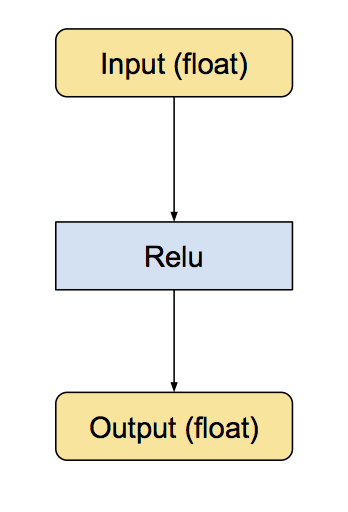
\includegraphics[scale=0.5]{quantization0.png}
\end{figure}
\end{center}
然后相应的转换子图,仍然是浮点输入输出,内部转换完成后以8位计算:
\begin{center}
\begin{figure}[H]
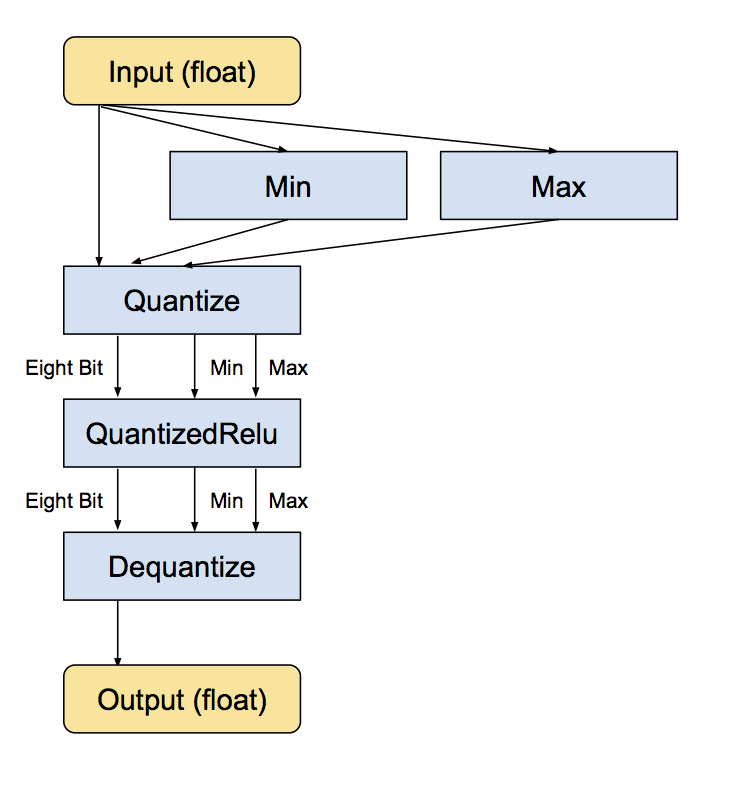
\includegraphics[scale=0.5]{quantization1.png}
\end{figure}
\end{center}
最小,最大操作实际上查看输入浮点tensor的值,输入他们到量化操作转换tensor为8位。

当单个操作被转换后,下一步是移除必要的转换到浮点。如果有一个连续的序列操作,将有一些链接Dequantize/Quantize操作

\begin{center}
\begin{figure}[H]
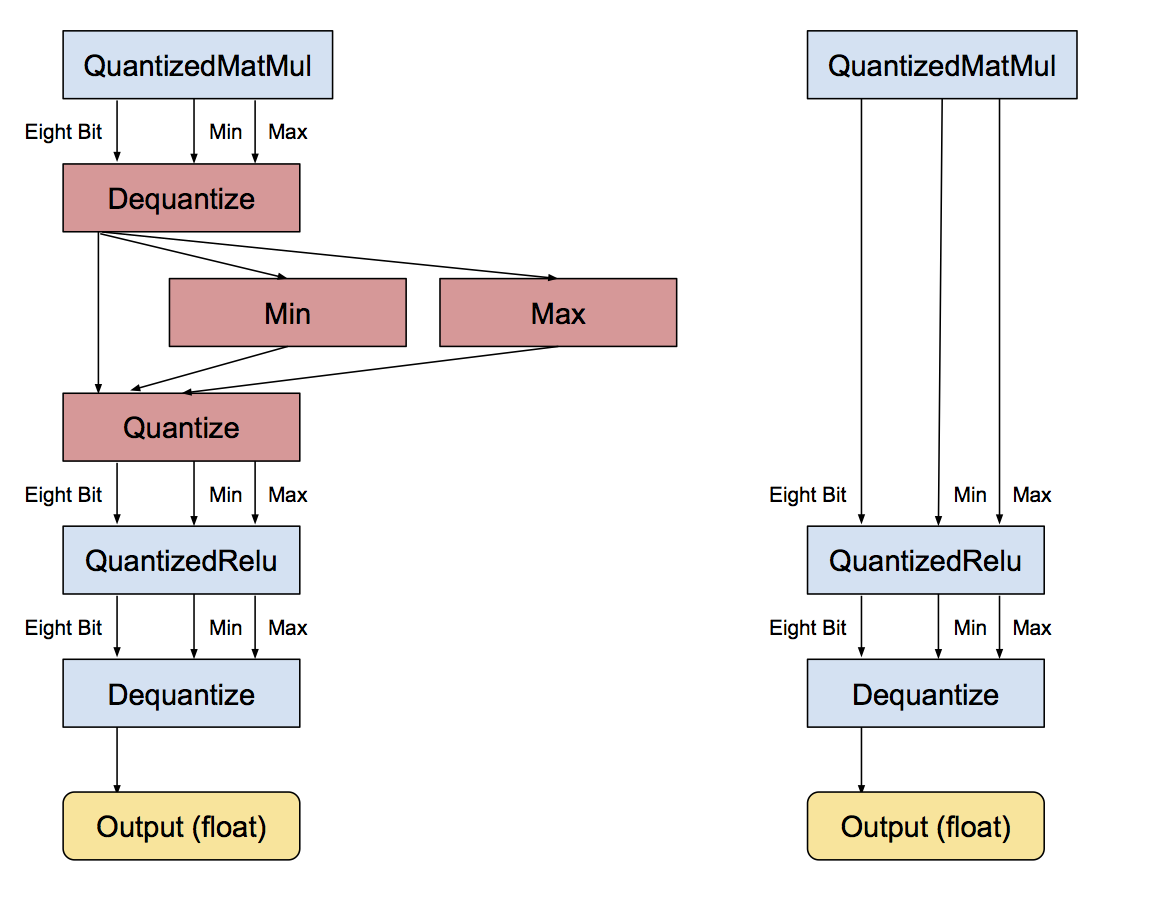
\includegraphics[scale=0.3]{quantization2.png}
\end{figure}
\end{center}
应用到大规模模型上时所有的操作已经相应的量化,图上所有的计算用8为计算不转换为浮点数。
\subsection{量化Tensor将呈现什么}
我们通过转化浮点数组为8位表达式作为压缩问题。我们知道权重和激活Tensor在训练神经网络模型时值的分布在一个小的范围(你也许有一个-15到+15的权重,-500到1000激活)。在实验中我们了解到神经网络通常在处理噪声时非常健壮,由量化产生噪声类似的误差将不会伤害精度。我们像卷则一个表达式这是容易执行计算,特别是大的矩阵惩罚影城需要运行一个模型的块。

这导致我们选择一个表达式有两个浮点数存储最小值和最大值代表最低和最高量化精度,每个在量化数组中的入口代表一个浮点值范围,现行飞蛾分布在最小值和最大值之间。例如我们有最小值=-10.0和最大值30.0f,和8位数据,下面是量化表达式:\newline
\begin{tabular}{|c|c|}
量化值&浮点数\\
0&-10\\
255&30.0\\
128&10.
\end{tabular}
\newline
这种表达式的好处是可以代表任一幅度的范围,我们不必须退成,它可以代表有符号和无符号的值,现行扩展使得直接相乘。对转换浮点数前后的一个清晰明确的量化格式定义好处,或者基于调试目的的查看tensor在Tensorflow上一个是线细节时希望提高将来最小值和最大值需要传递分割开得Tensor保持量化值,因此图个变得一点稠密。

最小和最大值范围可以提前计算,权重参数是常数在载入时就知道,因此他们的范围可以作为常数被存储。我们经常知道输入范围例如(RGB的值在0-255),一些激活函数也知道范围。这可以避免必须分析操作的输出决定范围,我们需要从8位输出像卷积或者矩阵乘法这样的做数学操作形成32Bit累加结果。
\subsection{下一步}
我们发现通过8为算法而不是不浮点数可以在移动短和嵌入式设备上得到机器好的性能。你可以看到这个框架我们优化矩阵乘在\href{https://github.com/google/gemmlowp}{gemmlowp},我们仍然需要应用所有的我们需要学习的TensorFlow操作去在移动短得到最大型能,但是我们很兴奋正在为次努力。马上,量化实现是一个合理的快和精确度实现我们希望将能在更多的设备上广泛的支持8位模型。我们也希望着站时将鼓励社区探索更低精度的神经网络的可能性。

